\documentclass{article}

% ready for submission
\usepackage[final]{neurips_2024}


% to compile a preprint version, e.g., for submission to arXiv, add add the
% [preprint] option:
%     \usepackage[preprint]{neurips_2024}


% to compile a camera-ready version, add the [final] option, e.g.:
%     \usepackage[final]{neurips_2024}


% to avoid loading the natbib package, add option nonatbib:
%    \usepackage[nonatbib]{neurips_2024}


\usepackage[utf8]{inputenc} % allow utf-8 input
\usepackage[T1]{fontenc}    % use 8-bit T1 fonts
\usepackage{hyperref}       % hyperlinks
\usepackage{url}            % simple URL typesetting
\usepackage{booktabs}       % professional-quality tables
\usepackage{amsfonts}       % blackboard math symbols
\usepackage{nicefrac}       % compact symbols for 1/2, etc.
\usepackage{microtype}      % microtypography
\usepackage{xcolor}         % colors

\usepackage{graphicx} % Required for inserting images
\usepackage{amsmath}
\usepackage{subcaption} % Required for creating subfigures
\usepackage{booktabs} % Required for \toprule, \midrule, \bottomrule

\title{Performance Evaluation on Transformers augmented with Hebbian and Gradient based plasticity}
\author{Brianna Grissom \And Christina Wang}
\date{November 2025}

\begin{document}

\maketitle

%\section{Notes (commented out)}

% Simplified Explanation of Model Limitations

% Limited Learning During Inference: The models can only temporarily use new information they encounter. This new evidence is processed through short-lived activations within their self-attention mechanism.
% No Permanent Information Storage: Unlike biological systems, these models lack a specific way to store or solidify this new information for long-term use during inference. This means they cannot truly learn and remember new things as they process information [1].

% \begin{itemize}


%     \item They augment decoder-only Transformers with the Hebbian rule fast-weight component
%     \item Fast-weight component: parameters that change very quickly during a forward pass. This allows the model to adapt quickly to new information. This approach allows for in-sequence adaptation, meaning the model can learn and adjust its behavior within the context of the data it is currently processing, rather than only during training steps.
%     \item When Transformers are augmented with fast-weight components, the model undergoes a forward pass every time it encounters new data. This is a core aspect of how these components enable rapid, in-sequence adaptation. This contrasts with the 'slow weights' of the Transformer, which are updated by the outer loop's gradient descent during training. Specifically, within each sequence (referred to as the inner loop), the fast weights are initialized to zero at the beginning and then updated online at every step [3] [4]. This update occurs via either a neuromodulated Hebbian rule or a gradient-based plasticity rule [3].
%     \item Position-wise FF NNs have a plastic component. The plastic layer $l$ has weights $W_l(t) = \tilde{W}_l(t) + w_l(t).$
%     \begin{itemize}
%         \item Plastic layer: a modified position-wise  FF NN within a Transformer that has been augmented with a dynamic, adaptable component. The FF NN is able to adapt weights during inference.
%         \item $\tilde{W}_l(t)$ = static meta-trained weights optimized by an outer loop backpropagation process
%         \item $w_l(t)$ = fast weights initialized to 0 at the start of each new sequence (input stream), ensuring that the model starts with a 'clean slate' of dynamic memory for each new task or data stream, preventing carry-over of fast-weight adaptations from previous sequences. These are updated locally during the forward pass.
%     \end{itemize}
% \item This “plasticity” is like giving the network a tiny, fast-learning brain on top of its usual, slowly-trained brain.
% \item Inner Loop Processing
% \begin{itemize}
%     \item Within each new sequence, the model's inner loop mechanism is activated. This involves updating the fast weights at every step of the sequence using either a Hebbian or gradient-based plasticity rule \textbf{[}3\textbf{]}. This step-wise adaptation allows the Transformer to incorporate new information and learn within the context of that specific sequence.
% \end{itemize}
% \item Outer Loop Optimization
% \begin{itemize}
%     \item The static parameters of the Transformer, including self-attention matrices and layer-normalization weights, are optimized by an outer loop. This outer loop update occurs once per sequence, using the task loss accumulated across that sequence \textbf{[}1\textbf{]} \textbf{[}3\textbf{]}. This two-timescale optimization (fast weights within a sequence, static weights across sequences) is fundamental to the meta-training procedure. 
%     \item These weights are not reset to 0 for each new sequence. They are designed to learn general rules or knowledge that applies across many tasks or sequences.
%     \item The outer loop optimizes these static parameters to support the in-sequence adaptations performed by the fast weights \textbf{[}1\textbf{]}. At test time, these static parameters remain fixed, and only the fast weights are updated online \textbf{[}2\textbf{]} \textbf{[}3\textbf{]}.
% \end{itemize}
% \item In essence, a "new sequence" marks the boundary for a fresh episode of in-context learning, where the model's fast-weight memory is reset and then dynamically updated as it processes the incoming data stream.
% \item Training Phase (Meta-training)
% \begin{itemize}
%     \item During the training phase, both static and fast weights undergo changes, but through different mechanisms and timescales:
%     \item Fast Weights: Within each sequence (the inner loop), the fast weights are initialized to zero at the start and then updated at every step using either a Hebbian or gradient-based plasticity rule. This allows for in-sequence adaptation. \textbf{[}1\textbf{]} \textbf{[}2]
%     \item Static Weights: Across sequences, an outer loop optimizes the static parameters and connection-specific learning rates to minimize the overall meta-loss. This means static weights are indeed updated during the training phase, but less frequently than fast weights, and their updates are designed to support the in-sequence adaptations performed by the fast weights. \textbf{[}1\textbf{]} \textbf{[}2]



%     \end{itemize}
%     \item Testing Phase: In the testing phase, the behavior of the weights changes significantly.
%     \begin{itemize}
%         \item Static weights: The static weights remain fixed and are \textit{not} updated. \textbf{[}3\textbf{]} This is because at test time, no outer-loop updates are applied.
%         \item Fast weights: The fast weights continue to be updated online for each new sequence through the model's in-sequence plasticity mechanisms. They are initialized to zero at the start of each new sequence and then dynamically updated as the sequence unfolds, enabling the model to adapt to new information without altering its static parameters.
%     \end{itemize}
% \item In essence, the training phase involves a two-timescale optimization where both types of weights are learned, with static weights learning general principles and fast weights learning how to adapt rapidly within a sequence. In contrast, the testing phase leverages the learned static weights as a stable foundation, while relying solely on the fast weights for dynamic, sequence-specific adaptation.
% \item At each step, model outputs token prediction $y_t$ and $(\tilde{\eta}_t, \bar y_t)$ that control the modulation signal $\eta(t)$, a learned signal that controls when and how strongly the fast weights are updated, allowing for gated and context-dependent plasticity. It influences $\eta(t)$. It is an internal LR.
% \begin{itemize}
%     \item $\tilde{\eta}_t$ = a pre-sigmoid scalar value that acts as a neuromodulation signal. It plays a role in determining when and how strongly plasticity is active, influencing the update of fast weights
%     \item $\bar y_t$ = a vector produced by a small head alongside the token prediction.
% \end{itemize}
% \item Hebbian Plasticity:  a biologically inspired mechanism that allows fast weights to adapt based on correlated pre- and post-synaptic activity. This rule enables the network to form and gate short-term associations based on contextual relevance.
% \begin{itemize}
%     \item Let $p_l(t)$ be the layer input and $q_l(t)$ be the post-synaptic activations (layer output).
%     \item Hebbian update for the weights is: $\Delta w_l(t) = (p_l(t)q_l(t)^T)$. 
%     \item  hollow dot = element-wise (Hadamard) product
%     \item Neuromodulation factor is $\eta(t) = \eta_0 \sigma(\tilde{\eta}_t)\times \,
% \min\left(1, \frac{\text{max\_norm}}{\lVert \delta_t \rVert_2}\right)$.
% \item $\eta_0$ = scalar hyperparameter, controls maximal LR
% \item $\sigma(\tilde{\eta}_t)$ = The sigmoid function applied to $\tilde{\eta}_t$ , which is a pre-sigmoid scalar neuromodulation logit.
% \item max\_norm: A constant used to clip the update magnitude. Contributes to the stability of the Hebbian update process, preventing overly aggressive or unstable changes to the fast weights. This helps in maintaining controlled adaptation within the Transformer model.
% \item $||\delta_t|| $ = The L2 norm of the vector $\delta_t$, which is formed by concatenating the flattened outer product of pre- and post-synaptic activities across all plastic layers. This mechanism allows the network to form and gate short-term associations based on contextual relevance, where Hebbian updates are sharply gated around salient events \textbf{[}1\textbf{]}. Forms a comprehensive signal used to determine when and how strongly plasticity should occur. Encodes the \textbf{candidate Hebbian weight change pattern} over all plastic layers at time t.
% \item when a pre-synaptic neuron and a post-synaptic neuron are active simultaneously, their connection strength (fast weight) is modified. This local adjustment is a key characteristic of biologically inspired plasticity. This makes the neuron become more sensitive to that input component in the future.
% \end{itemize}
% \item Experiments test two hypotheses: (1) How well the model can remember recent information (short-term memory) and (2) how well the model can quickly learn a new rule as it processes a single sequence.
% \item Experiment 1, Copy task (short term-memory task): The Transformer model is presented $n$ tokens, is shown 20 distractor inputs, and has to predict the original $n$ tokens again.
% \begin{itemize}
%     \item Expected result (what we're expected to get when we run their code): Plastic Transformer for both Hebbian and gradient update perform better than the standard Transformer. Gradient transformer does the best.
% \end{itemize}
% \item Experiment 2 ,  one-shot image classification (in-sequence learning task): Transformer sees a labeled image belonging to one of 5 classes and has to predict the class on 5 unlabeled images.
% \begin{itemize}
%     \item It sees pairs (image, label) for each class in random order. It is able to update plastic weights.
%     \item Then it sees one unlabeled image per class and has to predict the class using what it just learned.
%     \item First see \textit{one labeled example of each of the 5 classes}, then see a stream of unlabeled images from those same 5 classes and classify each as it arrives.
%     \item It does this in "episodes": each episode is the 5-class classification problem. After an episode, the static weights are updated. 
%     \item Support phase (labeled images): model sees $N \times K$ labeled examples, N=5 and K = 1. Input is [embedding, 1-hot-label, 0]. 0 means it's a support examples. The model only uses these steps to \textbf{update its fast (plastic) weights} and build an internal representation of the 5 classes.
%     \item Query phase (unlabeled images): model sees $N \times Q$ unlabeled images from the same 5 classes. Input is [embedding, 0, 1]. At every query step the Transformer outputs class scores (logits). \textbf{Cross-entropy loss is computed only here}, using the true class of each query image.
%     \item Use validation accuracy as a metric.
%     \item Expected results: Hebbian performs the best
% \end{itemize}
% \item Hebbian Plasticity dominates in situations with small datasets because the outer product weight update is like \textbf{writing a memory of the support example straight into the weights}. So each labeled example seen in the support phase becomes a little stored pattern the network can later match against when it sees query inputs. The neuromodulation factor is relatively small, meaning that it does not require huge plasticity signals to work.
% \end{itemize}

\section{Background}
\noindent
The strong capability and potential of Transformers has been proven by the extensive computational analysis done by OpenAI. When increased to a very large scale (from 125M to 175B parameters), transformers are capable of generalizing NLP tasks after training on a large and extensive dataset, without extensive task-specific finetuning \cite{gpt3}. Thus, a lot of research has been trying to either investigate the learning abilities of the transformer model, or aiming to improve their architecture so that they learn more efficiently.

One thing Transformers, or all general machine learning models suffer from is the inefficiency to quickly process new information that can be derived from already learned data after post-training.

Inspired by the famous Hebbian Plasticity Rule that updates weights synchronously every time it encounters new data, Duan et al researches on the prospect of implementing plasticity on RNN models, based on both the famous Hebbian plasticity rule and their newly proposed plasticity rule derived from Gradient descent. \cite{duan2023hebbiangradientbasedplasticityenables}

The project done by Siddharth Chaudhay then follows up their work by implementing both the Hebbian and Gradient plasticity rule on decode-only Transformers, and does a computational test of several tasks to investigate their performance.\cite{chaudhary2025enablingrobustincontextmemory}

In this report, we will first introduce the Hebbian and Gradient Plasticity rules and its implementation, then follow up the work of Siddharth Chaudhay and design more tests to evaluate and compare the performance of the two models.

\section{Hebbian \& Gradient Plasticity}

The inability of Transformers to permanently store new information encountered post-training does not allow them to learn new things. To solve this problem, decoder-only Transformers are augmented with a fast-weight component that allow for in-sequence adaption, meaning that the model can adjust its behavior quickly as it processes new data. \vspace{3pt}

In the training stage, the model undergoes forward passes that updates its fast weights every time it encounters new data, also known as the "inner loop". Meanwhile, the Transformer's static weights are updated via gradient descent at a much less frequent rate, also known as the "outer loop". \vspace{3pt}

\noindent
In the testing stage, the static weights remain fixed while the fast weights, initialized to zero at the start of each new sequence, continue to be updated for each new sequence through the model's in-sequence plasticity mechanisms. This allows the model to adapt to new information and learn  within the context of that specific sequence while keeping the static weights fixed. \vspace{3pt}


The position-wise feed-forward neural networks have the weight matrix $$W_l(t) = \tilde{W}_l(t) + w_l(t)$$ for each plastic layer $l$, where $\tilde{W}_l(t)$ are the static meta-trained weights optimized by an outer loop backpropagation process and $w_l(t)$ are the fast weights initialized to zero at the start of each new sequence and are updated locally during the forward pass. The inner loop does its fast weight updates using either a Hebbian or a gradient-based plasticity rule.\vspace{10pt}

\noindent
Figure 1 presents pseudocode for the training algorithm \cite{chaudhary2025enablingrobustincontextmemory}.

\begin{figure}[h]
\centering
\includegraphics[scale=0.4]{training-algorithm.png}
\caption{Pseudocode for Training Algorithm}
\label{pseudocode}
\end{figure}

\noindent
$\alpha_l$ is a connection-specific learning rate and $\eta(t)$ represents the modulation signal that controls how strongly the fast weights are updated, allowing for context-dependent plasticity. At each step, the model outputs the token prediction $y_t$ and variables $(\tilde{\eta}_t, \bar y_t)$ that control the modulation signal $\eta(t)$. $\tilde{\eta}_t$ acts as a neuromodulation signal and $\bar y_t$ is a vector produced by a small head alongside the token prediction.\vspace{10pt}

\noindent
\textbf{Hebbian Plasticity Rule}\vspace{5pt}

\noindent
Hebbian Plasticity is a biologically inspired mechanism that updates the fast weights based on pre- and post-synaptic activity correlations. This allows the Transformer to store short-term associations. Let $p_l(t)$ denote the input (the pre-synaptic activations) and $q_l(t)$ denote the layer output (the post-synaptic activations)  for layer $l$ of the feed forward neural network. The Hebbian plasticity update for the fast weights is $$\Delta w_l(t) = (p_l(t)q_l^T(t)),$$  where the neuromodulation factor $\eta(t)$ is $$ \eta(t) = \eta_0 \sigma(\tilde{\eta}_t)\times \, 
\min\left(1, \frac{\text{max\_norm}}{\lVert \delta_t \rVert_2}\right)\; \text{and}\;$$ 

$$\delta_t = \text{Concat}\bigl(\text{Vec}(p_l(t) q_l^\top(t)) \mid l \in S\bigr).$$ 

$\eta_0$ is a scalar hyperparameter than controls the maximal learning rate, $\sigma(\tilde{\eta_t})$ is the sigmoid function applied to $\tilde{\eta}_t$, max\_norm is a constant used to prevent aggressive or unstable changes to the fast weights, and $\delta_t$ encodes the Hebbian weight change pattern over all plastic layers at time $t$. 

\noindent
Interpretation: Strong correlations between pre-synaptic and post-synaptic neurons captured in the dot product term indicate that their connection strength (fast weight) is modified significantly, making the neuron become more sensitive to that input component in the future. \vspace{10pt}

\noindent
\textbf{Gradient Plasticity Rule}\vspace{5pt}

\noindent
Gradient Platicity is a modern framework that makes use of gradient descent on global information to update the pre- and post-synaptic weights \cite{duan2023hebbiangradientbasedplasticityenables}. For a customized global loss function $L$,
\noindent
The update for each weight vector:

$$\Delta w_l(t) \propto \frac{\delta L}{\delta w_l}$$
\noindent

While the traditional Hebbian rule does not care about a bias term $b$ present in each layer of the network, the Gradient rule by Duan et al also adds plasticity to the bias term:

$$\Delta b_l(t) \propto \frac{\delta L}{\delta b_l}$$
\noindent

The neuromodulation factor $\eta(t)$ is derived similarly as the the Hebbian Plasticity Rule.


\section{Experiments}

The following experiments will test two hypotheses: 
\begin{enumerate}
    \item How well the model can remember recent information (short-term memory)
    \item How well the model can quickly learn a new rule as it processes a single sequence (rapid, in-sequence learning)
\end{enumerate}
\vspace{10pt}

Each experiment is run with $S=3$ seeds and reported metrics are mean $\pm$ standard deviation across seeds. 

During training, the fast weights are updated every step via the Hebbian or gradient rule and the static weights are updated once per sequence using the task loss accumulated across that sequence.

During testing, the models adapt only through the fast weights.


\subsection{Reproduced Experiments}

\subsubsection{Copy Task}

\noindent
In this task, the Transformer model first is presented $n$ tokens, then is shown 20 distractor inputs which are all blank tokens. Finally, it has to predict the original $n$ tokens again. This is an example of a short-term memory task. 

The metrics tracked here are validation loss and recall accuracy. Their experiment uses 50 episodes per epoch for 2 epochs with state reset between sequences. 

The results are shown together with the next experiment in table \ref{tab:reproduced_results} and figure \ref{fig:Experiment_1_2_results}. 

\subsubsection{One-Shot Image Classification}

\noindent
This experiment is an image classification task on the CIFAR-FS and Omniglot datasets, representing rapid, in-sequence learning. 

There are two phases of this experiment: support and query. 

In the Support Phase, the Transformer sees $N \times K$ labeled examples, where $N = 5$ and $K = 1$. The labeled examples take the form [embedding, one-hot-label, 0], where 0 means it’s a support example. In this phase, the model uses the data to update its fast (plastic) weights to build an internal representation of the 5 classes.

In the Query Phase, the model sees $N \times Q$ unlabeled images from the same $N=5$ classes of the form [embedding, 0, 1]. At every query step the Transformer outputs class scores (logits) and cross-entropy loss is computed using the true class of each query image. Validation accuracy is used as a metric. 

They repeat this for a number of episodes, where new images are sampled. After an episode, the static weights are updated.

Eighty and 100 classification episodes per epoch are used for Omniglot and CIFAR-FS, respectively, for a total of 5 epochs. The number of inner updates per episode is $N \times K$ (support) + $N \times Q$ (queries).

The results are shown together as the copying experiment in table \ref{tab:reproduced_results} and figure \ref{fig:Experiment_1_2_results}. 

\subsubsection{Results}
The results from the original paper are shown in Figure \ref{original_accuracy} and Table \ref{tab:original_results}: The accuracy for the copying task is almost uniform across models, and it appears that the Hebbian Plasticity rule performs the best for image classification. 

The reproduced accuracy as of Figure \ref{reproduced_accuracy} and Table \ref{tab:reproduced_results} exhibits the same behavior for the copying task. For image classification, Hebbian is still the best for the Omniglot Dataset. In our CIFAR-FS case, however, perhaps due to the inherent randomness of testing, the baseline Transformer without any plasticity rule seems to perform the best.

The neuromodulation and the plastic weight norm are of similar scale compared to the results of the original paper.

\begin{table}[t]
\centering
\caption{Performance across tasks (mean $\pm$ std over 3 runs) from original paper}
\label{tab:original_results}
\begin{tabular}{l c c c}
\toprule
Rule
& CIFAR-FS Acc.  
& Omniglot Acc. 
& Copy Recall \\
\midrule
None
& 0.289 $\pm$ 0.028
& 0.192 $\pm$ 0.020
& 0.721 $\pm$ 0.025 \\

Hebbian
& \bf{0.319 $\pm$ 0.017}
& \bf{0.237 $\pm$ 0.028}
& 0.727 $\pm$ 0.007 \\

Gradient
& 0.274 $\pm$ 0.038
& 0.201 $\pm$ 0.012
& \bf{0.745 $\pm$ 0.011} \\
\bottomrule
\end{tabular}
\end{table}


\begin{table}[t]
\centering
\caption{Reproduced Performance across tasks (mean $\pm$ std over 3 runs).}
\label{tab:reproduced_results}
\begin{tabular}{l c c c}
\toprule
Rule 
& CIFAR-FS Acc.  
& Omniglot Acc. 
& Copy Recall \\
\midrule
None     
& \bf{0.274 $\pm$ 0.034}
& $0.234 \pm 0.055$
& $0.774 \pm 0.002$ \\

Hebbian  
& $0.269 \pm 0.028$
& \bf{0.246 $\pm$ 0.054}
& $0.771 \pm 0.005$ \\

Gradient 
& $0.262 \pm 0.034$
& $0.236 \pm 0.066$
& \bf{0.774 $\pm$ 0.004} \\
\bottomrule
\end{tabular}
\end{table}

\begin{figure}[h]
    \centering
    % --- First Subfigure ---
    \begin{subfigure}[b]{\textwidth}
        \centering
        % Replace 'example-image-a' with your filename
        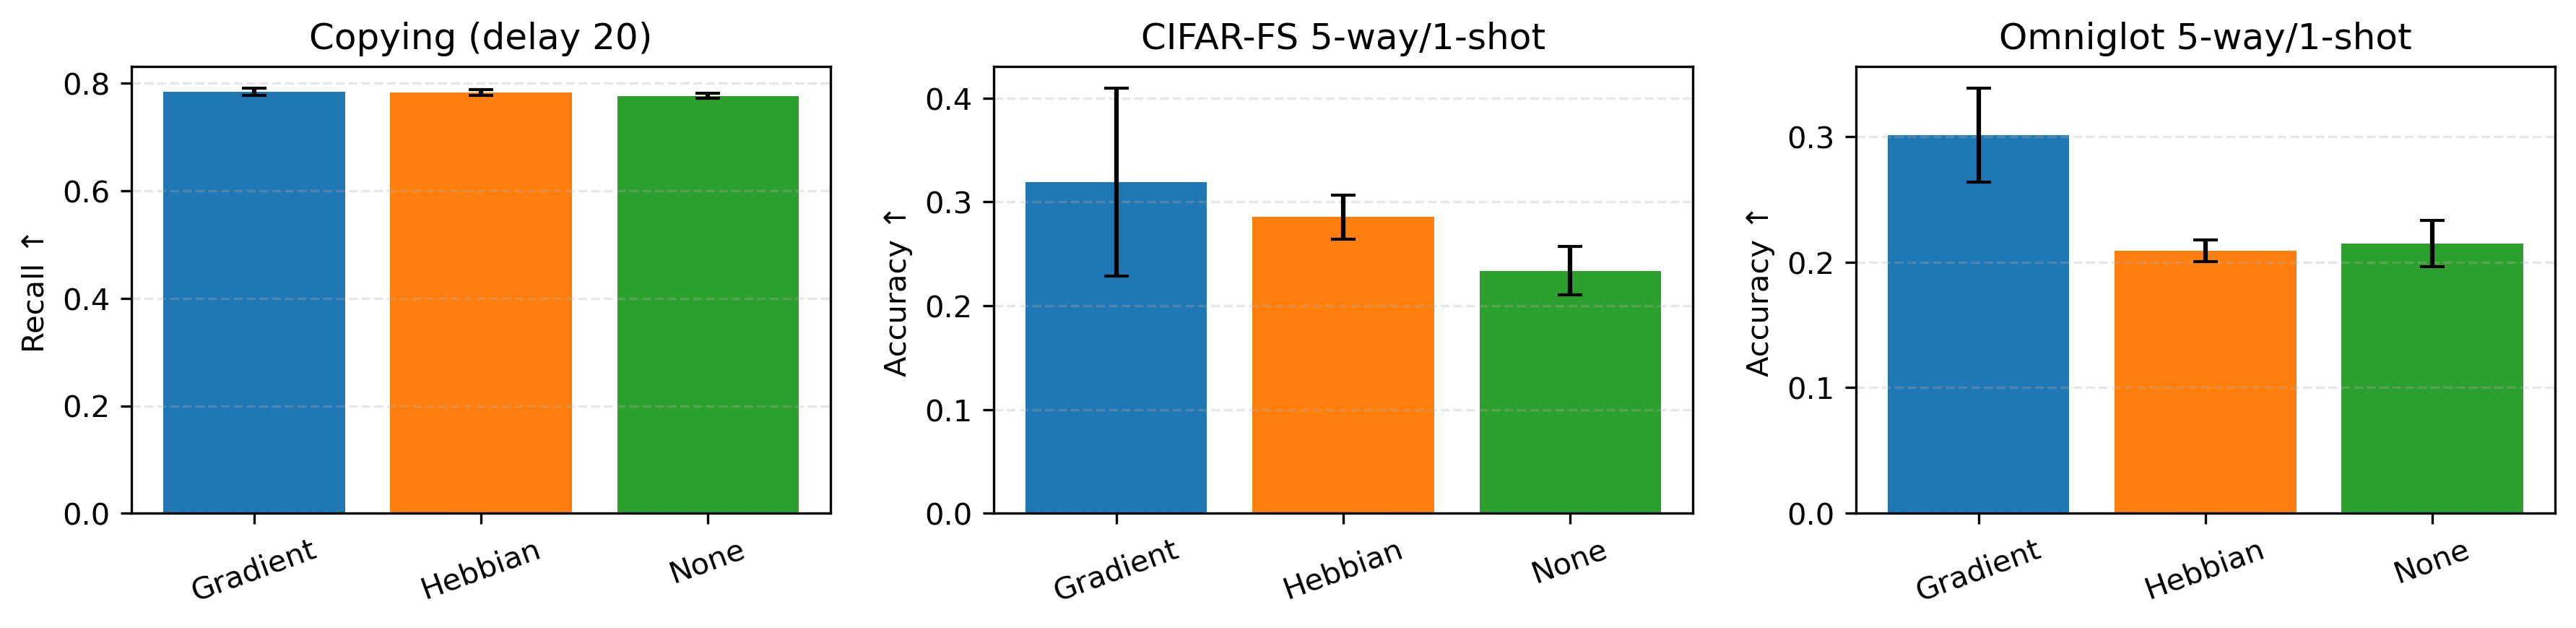
\includegraphics[width=\textwidth]{reproduction_figures/performance_accuracy.png}
        \caption{Reproduced Final Accuracy}
        \label{reproduced_accuracy}
    \end{subfigure}
    \hfill % Adds flexible space between images
    % --- Second Subfigure ---
    \begin{subfigure}[b]{\textwidth}
        \centering
        % Replace 'example-image-b' with your filename
        \includegraphics[width=\textwidth]{reproduction_figures/performance_accuracy_original.pdf}
        \caption{Final Accuracy in original paper}
        \label{original_accuracy}
    \end{subfigure}
    \hfill % Adds flexible space between images
    % --- Third Subfigure ---
    \begin{subfigure}[b]{0.4\textwidth}
        \centering
        % Replace 'example-image-c' with your filename
        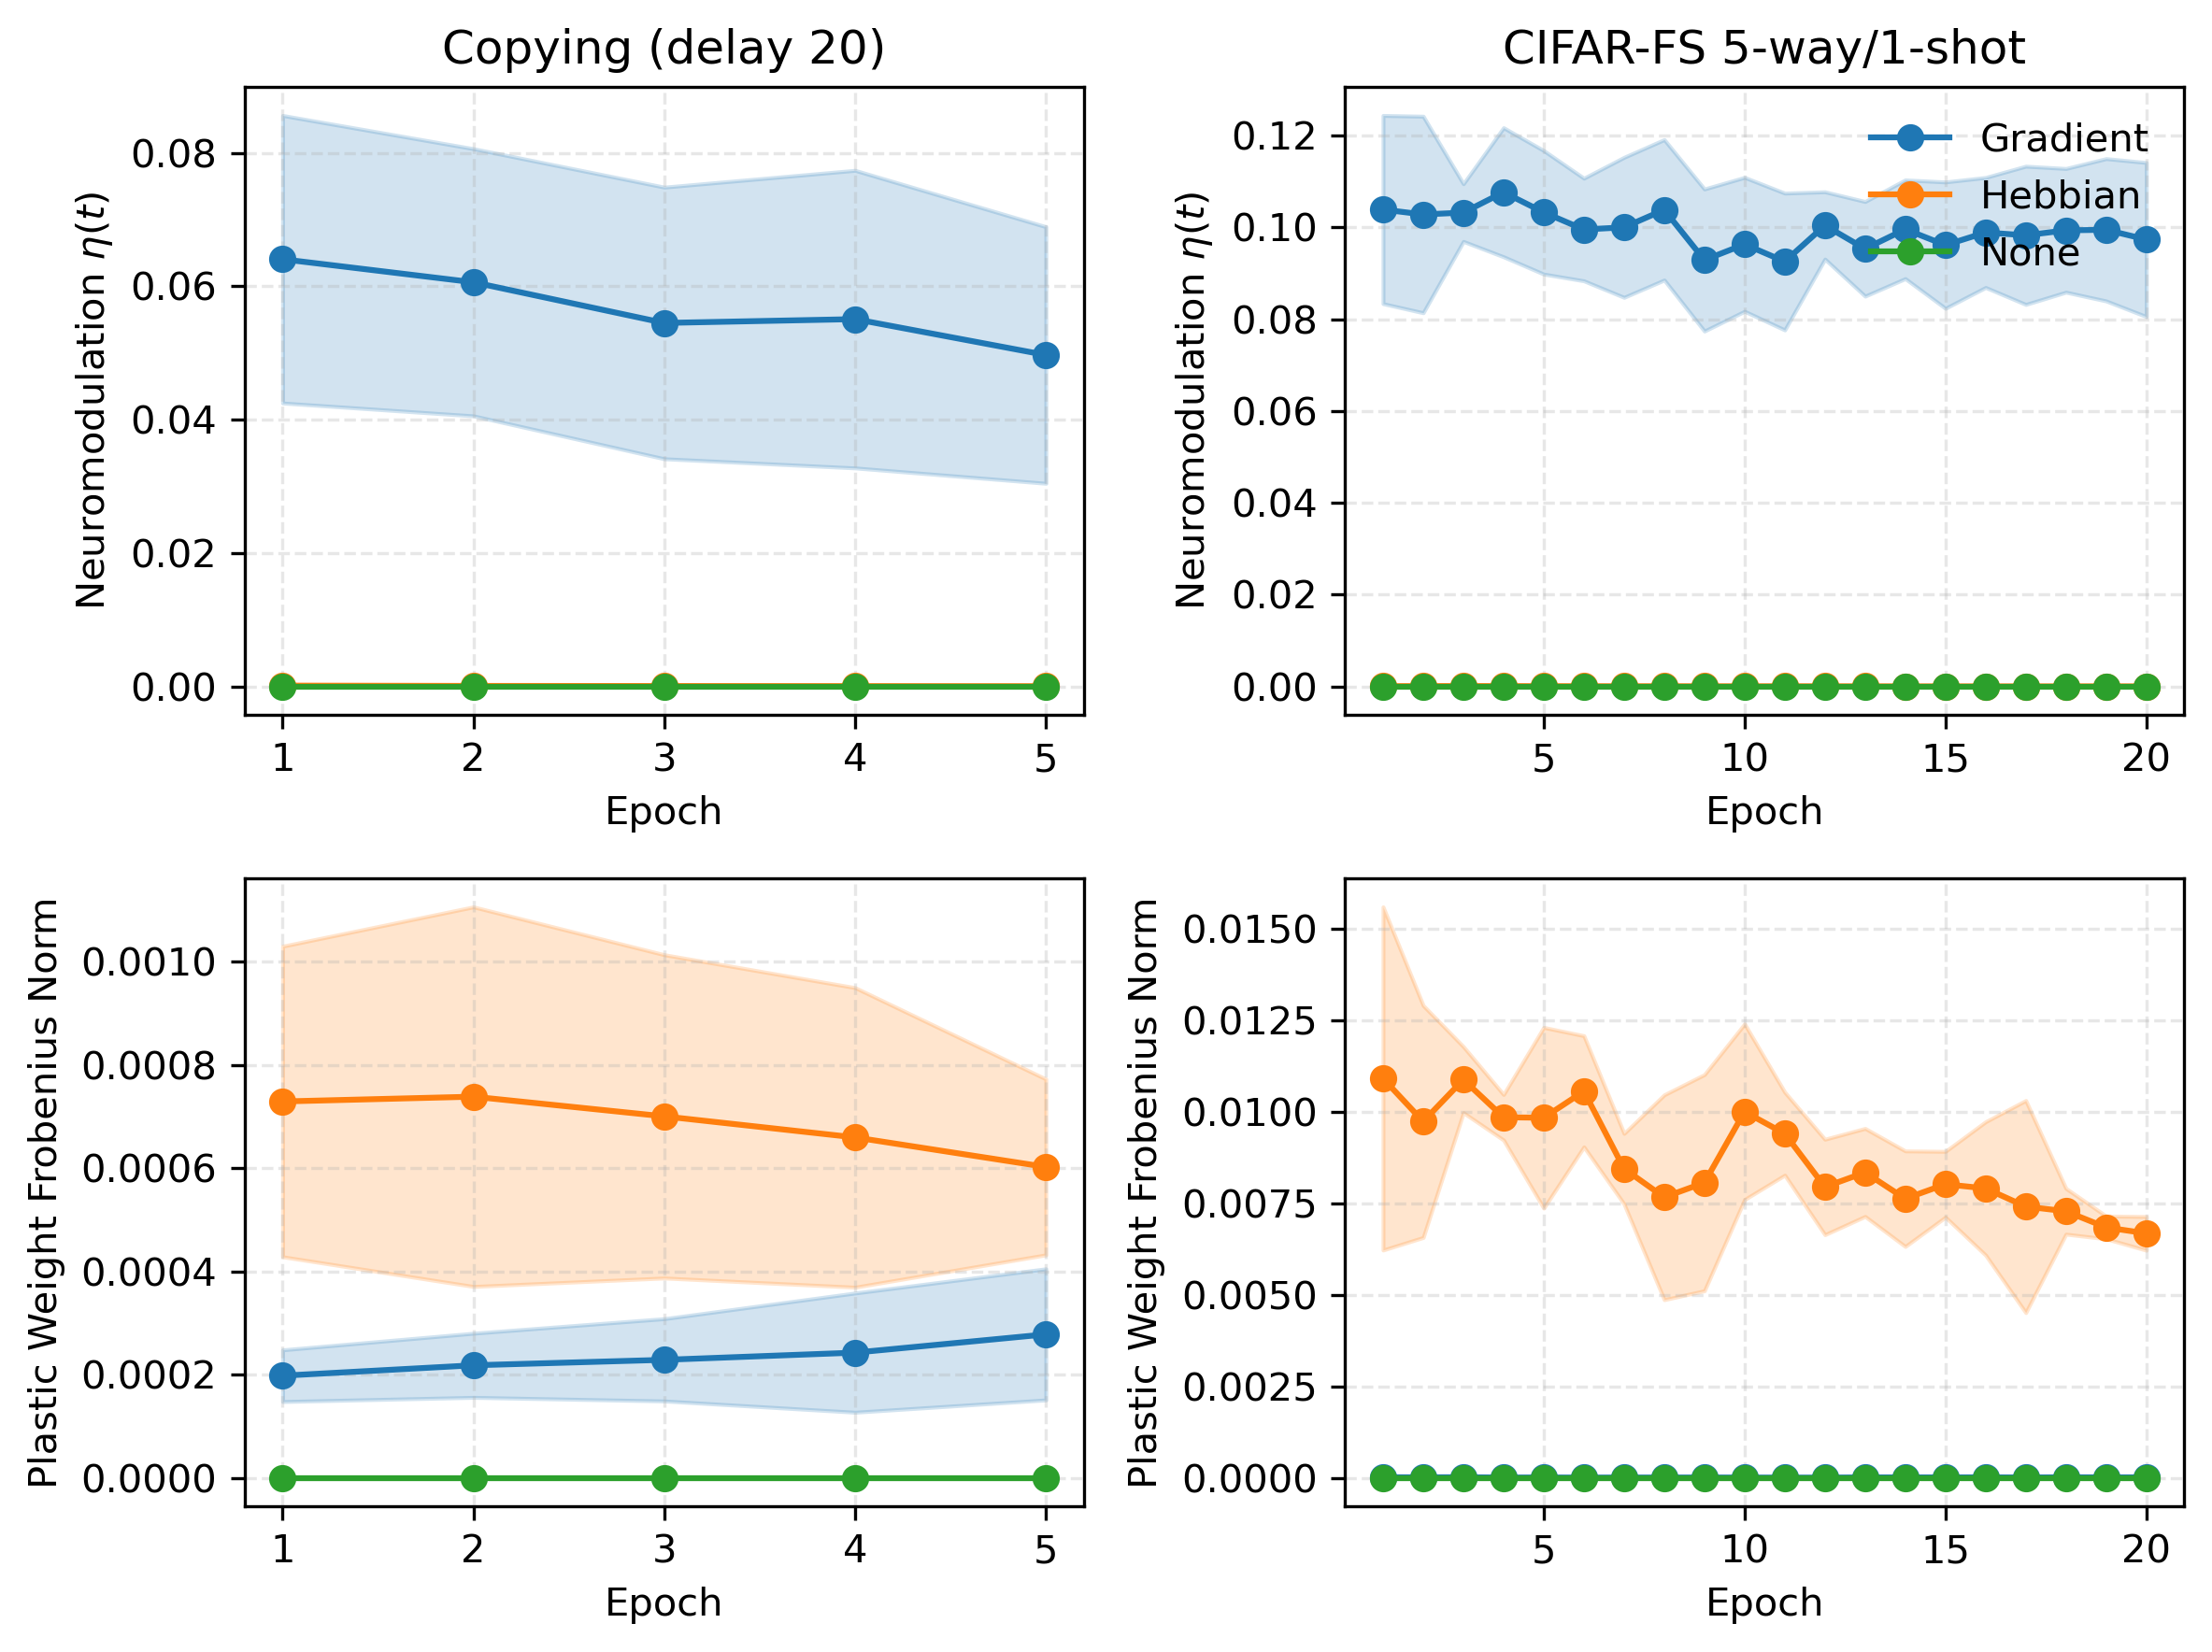
\includegraphics[width=\textwidth]{reproduction_figures/mechanistic_traces.png}
        \caption{Reproduced $\eta(t)$ and plastic weight norm}
        \label{reproduced_norms}
    \end{subfigure}
    \hfill % Adds flexible space between images
    % --- Third Subfigure ---
    \begin{subfigure}[b]{0.4\textwidth}
        \centering
        % Replace 'example-image-c' with your filename
        \includegraphics[width=\textwidth]{reproduction_figures/mechanistic_traces_original.png}
        \caption{$\eta(t)$ and plastic weight norm in original paper}
        \label{reproduced_norms}
    \end{subfigure}
    \caption{Results for Copy and Image Classification Experiment}
    \label{fig:Experiment_1_2_results}
\end{figure}

\subsection{Extended Reproduction Experiments}
From the original paper, we also extended their experiments in two ways.

1) We increased the training epochs from 2 to 5 in the copying task, and increased the training epochs for image classification from 5 to 20 and look at the results. The results are shown combined in Figure \ref{fig:Experiment_extended_results} and \ref{tab:img_copy_results}.

2) We tested the copying task for the three models with varying signal length, in order to see the memory capacity for different models while fixing the same model size and parameters. We train 5 epochs over each copying length and look at the models' final accuracy. The results are shown in Figure \ref{fig:copying_capacity_results}. 

Here, We limit the model to be of 2 layers, with 2 transformer blocks and 4 attention heads, 128 hidden parameters, and 0.1 dropout probability. This is consistent with their original test model for their copying experiments.


\subsubsection{Increased Training Epochs}
By simply increasing the number of epochs, we clearly see a discrepancy from the original paper's results. Here, the gradient model becomes the best one, with only slight win over in the copying task, and becomes significantly better than the other two in image classification. 

Neuromodulation and Plastic Weight Norms are on the same scale as shown before, indicating that the model is actively adapting to new information.

The original paper only ran 5 epochs using a very small model for the tasks, and especially for image classification, they stopped with a final classification accuracy only up to around 0.3. In real world scenarios, significantly larger models are used and being trained with significantly larger number of epochs. 

For consistency with the original paper's results, and due to limitation in time and resources, this extended performance test only increased the number of epochs. Even so, we see that the result looks significantly different. It is safe to say that the results obtained from the original paper would need more testing to hold better significance in real applications. 

%In our new experiment introduced later, we will use a larger model to run to get higher accuracy results.

\begin{figure}[h]
    \centering
    % --- First Subfigure ---
    \begin{subfigure}[b]{\textwidth}
        \centering
        % Replace 'example-image-a' with your filename
        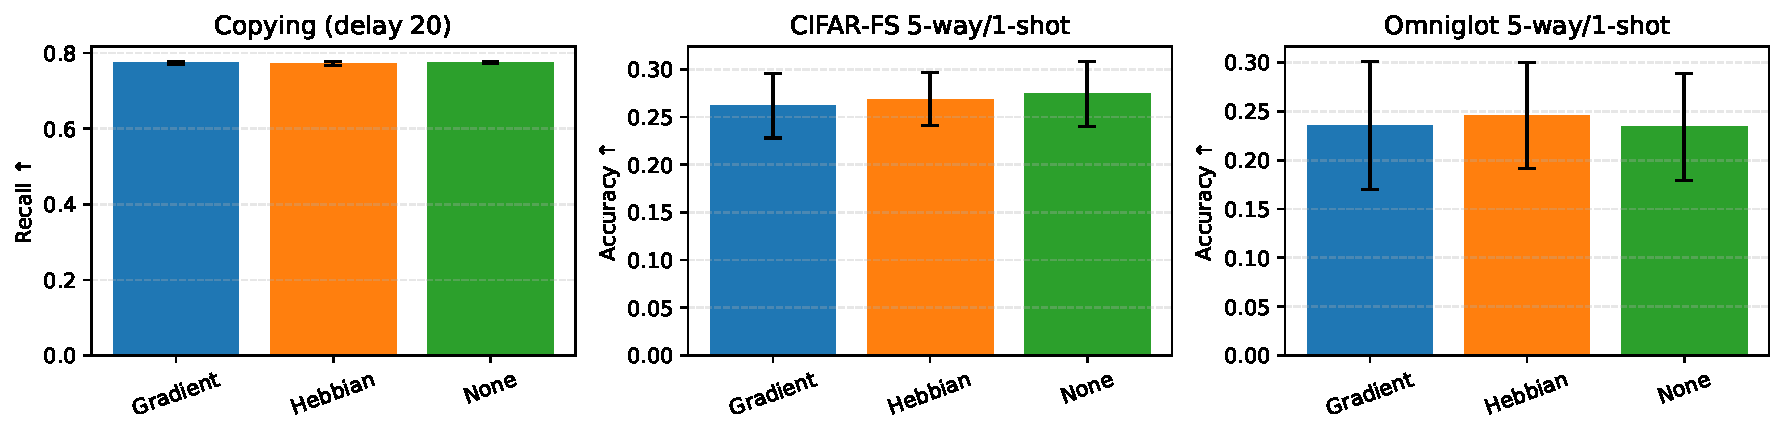
\includegraphics[width=\textwidth]{extended_figures/performance_accuracy.png}
        \caption{Final Accuracy after extended training}
    \end{subfigure}
    \hfill % Adds flexible space between images
    % --- Second Subfigure ---
    \begin{subfigure}[b]{0.7\textwidth}
        \centering
        % Replace 'example-image-b' with your filename
        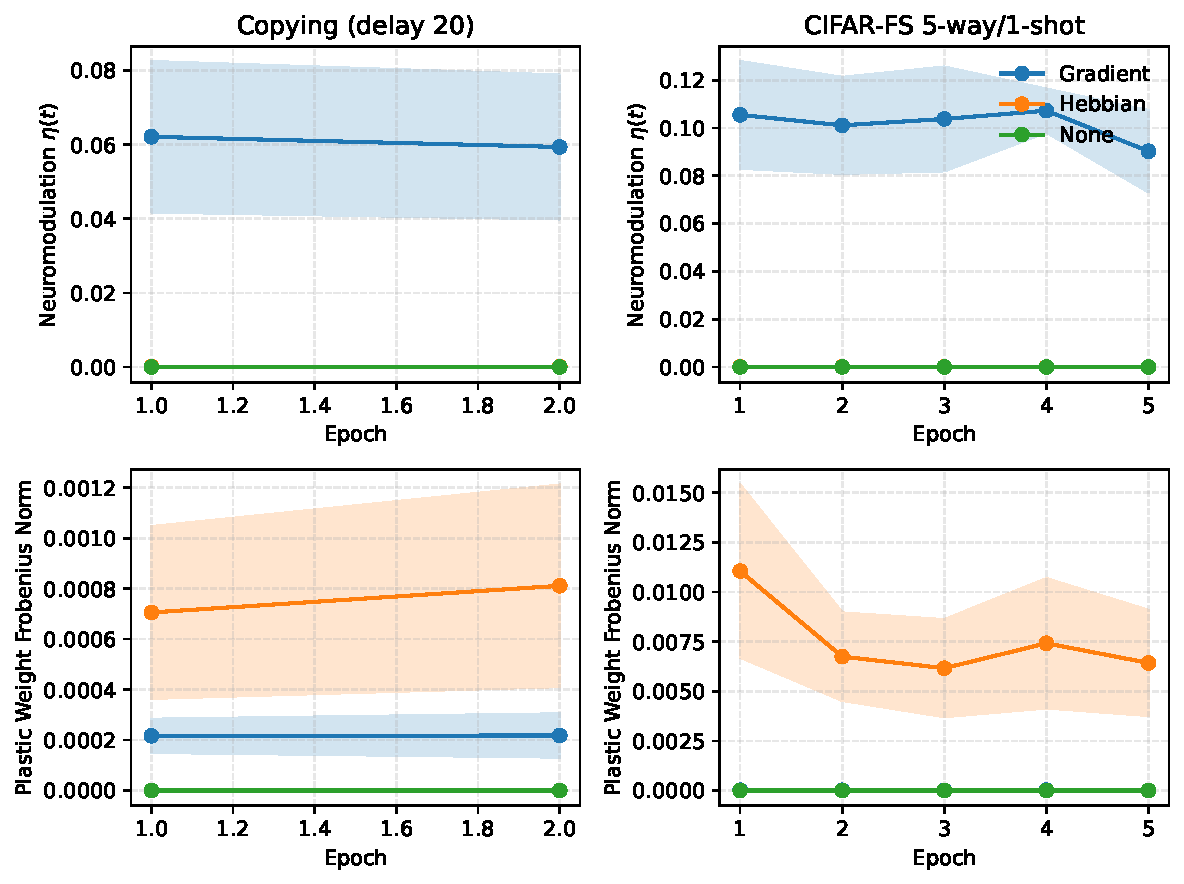
\includegraphics[width=\textwidth]{extended_figures/mechanistic_traces.png}
        \caption{$\eta(t)$ and plastic weight norm after extended training}
    \end{subfigure}
    \caption{Results for Copy and Image Classification Experiment after extended training}
    \label{fig:Experiment_extended_results}
\end{figure}

\begin{table}[t]
\centering
\caption{Extended Performance on image classification and copying tasks (mean $\pm$ std over 3 runs).}
\label{tab:img_copy_results}
\begin{tabular}{l c c c}
\toprule
Rule 
& CIFAR-FS Acc. 
& Omniglot Acc.  
& Copy Recall  \\
\midrule
None     
& $0.234 \pm 0.024$
& $0.215 \pm 0.018$
& $0.777 \pm 0.005$ \\

Hebbian  
& $0.286 \pm 0.021$
& $0.209 \pm 0.009$
& $0.783 \pm 0.005$ \\

Gradient 
& \bf{0.319 $\pm$ 0.091}
& \bf{0.301 $\pm$ 0.038}
& \bf{0.784 $\pm$ 0.007} \\
\bottomrule
\end{tabular}
\end{table}

\subsubsection{Copying Capacity testing}

By testing the copying task on a wide range of Signal Lengths, we see that due to the limitation of parameter sizes, the three models show similar decrease trends. 

However, we also see that the baseline Transformer has a significantly larger variance compared to the other two. By adding plasticity rules, in this scenario, the model seems to better adapt to randomness and exhibits stable behavior across different seeds.


\begin{figure}[h]
\centering
    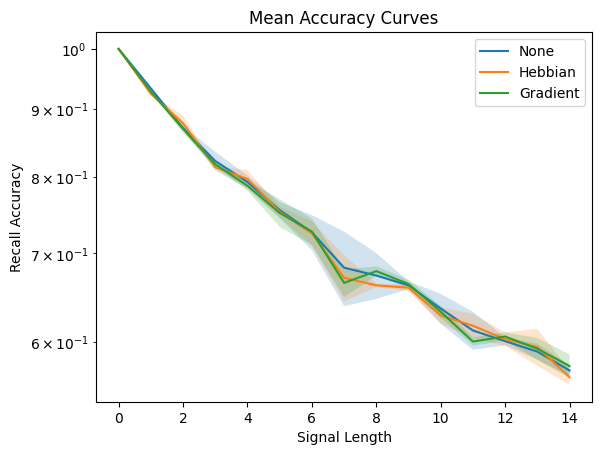
\includegraphics[width=0.5\textwidth]{extended_figures/output.png}
    \caption{Recall Accuracy for copying tasks graphed respect to signal length. the filled area is the $95\%$ Confidence Interval}
    \label{fig:copying_capacity_results}
\end{figure}

\subsection{New Experiment: Three-Shot Text Category Classification}

We created a text category classification task as another way to test rapid, in-sequence learning. Similar to the above design, we test a 3-way, 3-shot classification task, but this time with textual data. The model will be presented with words belonging to one of three categories: animals, furniture and clothing. Its goal is to predict which category a given word belongs to. Below are the ten words for each category:

\begin{itemize}
    \item Animals: "dog", "cat", "fish", "mouse", "deer", "bear", "wolf", "lion", "tiger", "elephant"
    \item Furniture: "table", "chair", "carpet", "couch", "bed", "desk", "shelf", "cabinet", "wardrobe", "dresser"
    \item Clothing: "shirt", "skirt", "jacket", "dress", "pants", "shorts", "shoes", "hat", "coat", "gloves"
\end{itemize}

For training, we provide 3 support words per class and test on 2 query words for each of the 3 classes for each episode. For word embeddings, semantic embeddings are used to ensure that words in each class are similar in embedding space and differ significantly from embeddings in other classes. An embedding for a word was calculated as

\textit{category\_base + word\_offset(word)}, where \textit{category\_base} is the base embedding vector for that category and \textit{word\_offset(word)} adds word-specific variation to that category. 

We train for 200 episodes and evaluate on 100 episodes for a total of 5 epochs. Our metrics are validation classification accuracy averaged across the 3 seeds (reported as mean $\pm$ standard deviation) and the plastic weight norm and $\eta(t)$ for the plastic model. \vspace{10pt}


\subsubsection{Results}

Table \ref{tab:Experiment 4 Table} displays the accuracy results and Figure \ref{fig:Experiment 4 Results}  displays an accuracy bar plot, accuracy across epochs, plot of the neuromoduluation factor, and plot of the plastic weight norm for this task. The values and associated error bars for each plot are calculated using the mean and standard deviation of the three different seeds.



\begin{figure}[h]
    \centering
    % --- First Subfigure ---
    \begin{subfigure}[b]{0.3\textwidth}
        \centering
        % Replace 'example-image-a' with your filename
        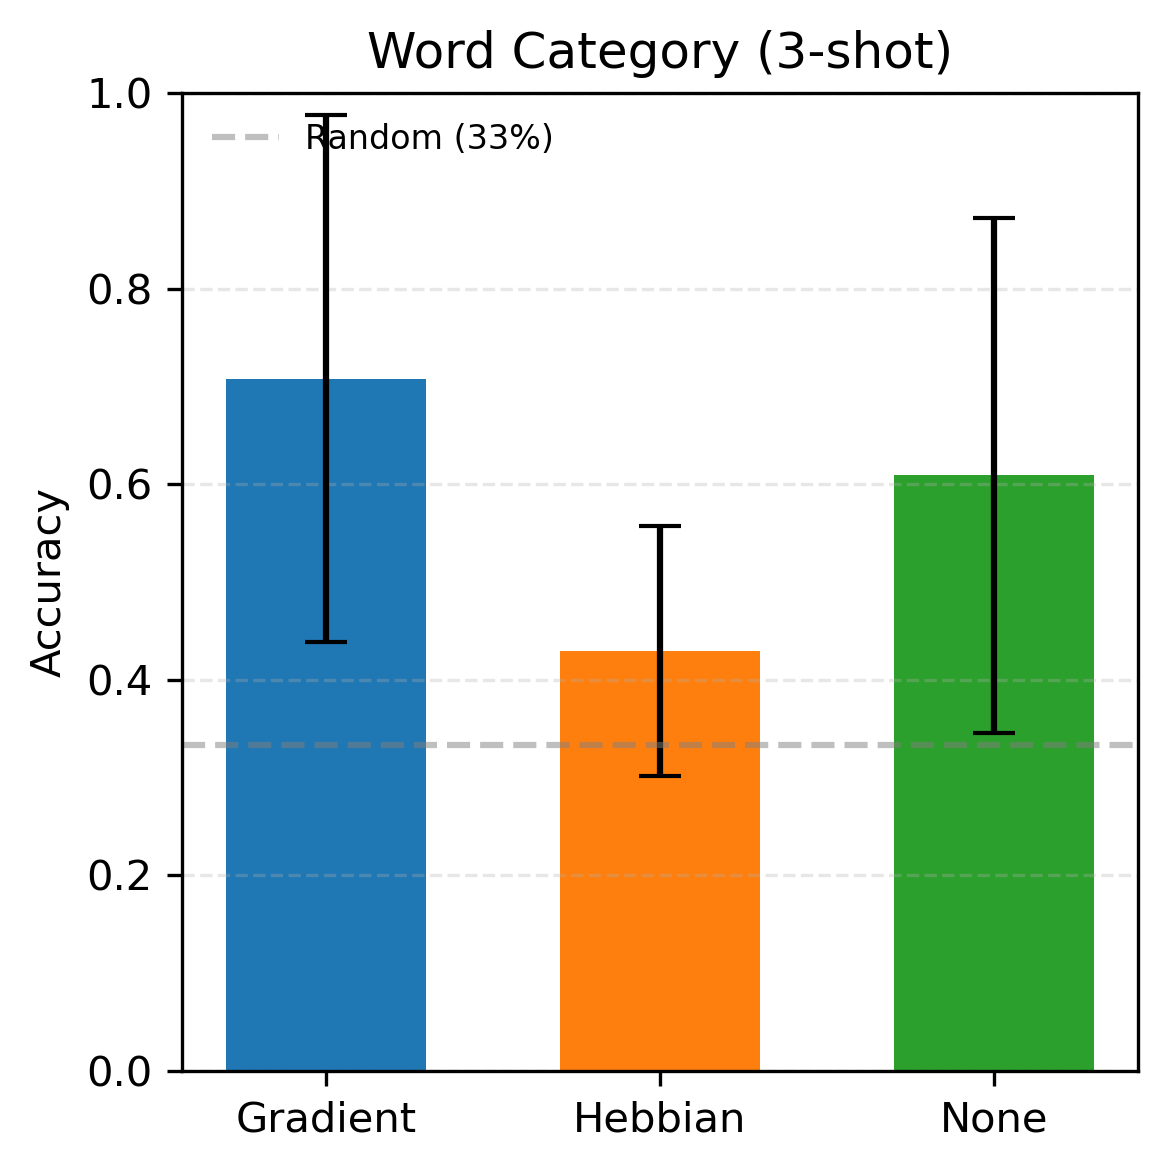
\includegraphics[width=\textwidth]{word_category_figures/word_category_accuracy_bars.png}
        \caption{Final Accuracy}
        \label{fig:plot1}
    \end{subfigure}
    \hfill % Adds flexible space between images
    % --- Second Subfigure ---
    \begin{subfigure}[b]{0.3\textwidth}
        \centering
        % Replace 'example-image-b' with your filename
        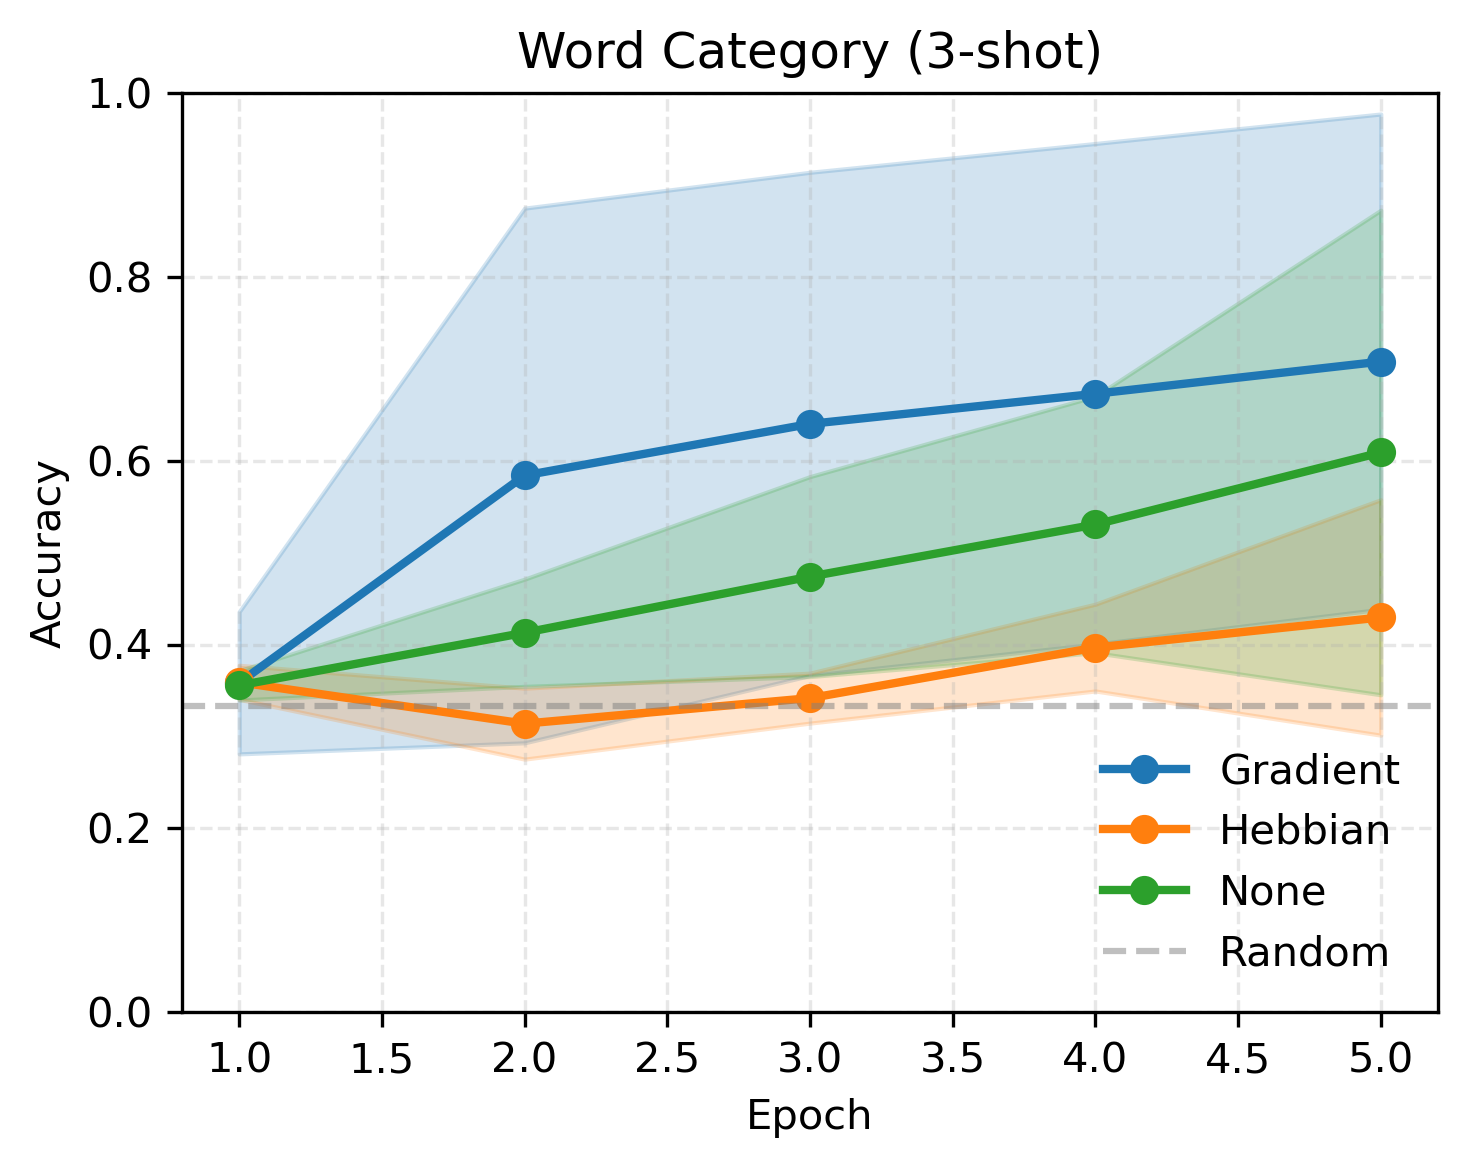
\includegraphics[width=\textwidth]{word_category_figures/word_category_accuracy_curves.png}
        \caption{Accuracy by epoch}
        \label{fig:plot2}
    \end{subfigure}
    \hfill % Adds flexible space between images
    % --- Third Subfigure ---
    \begin{subfigure}[b]{0.3\textwidth}
        \centering
        % Replace 'example-image-c' with your filename
        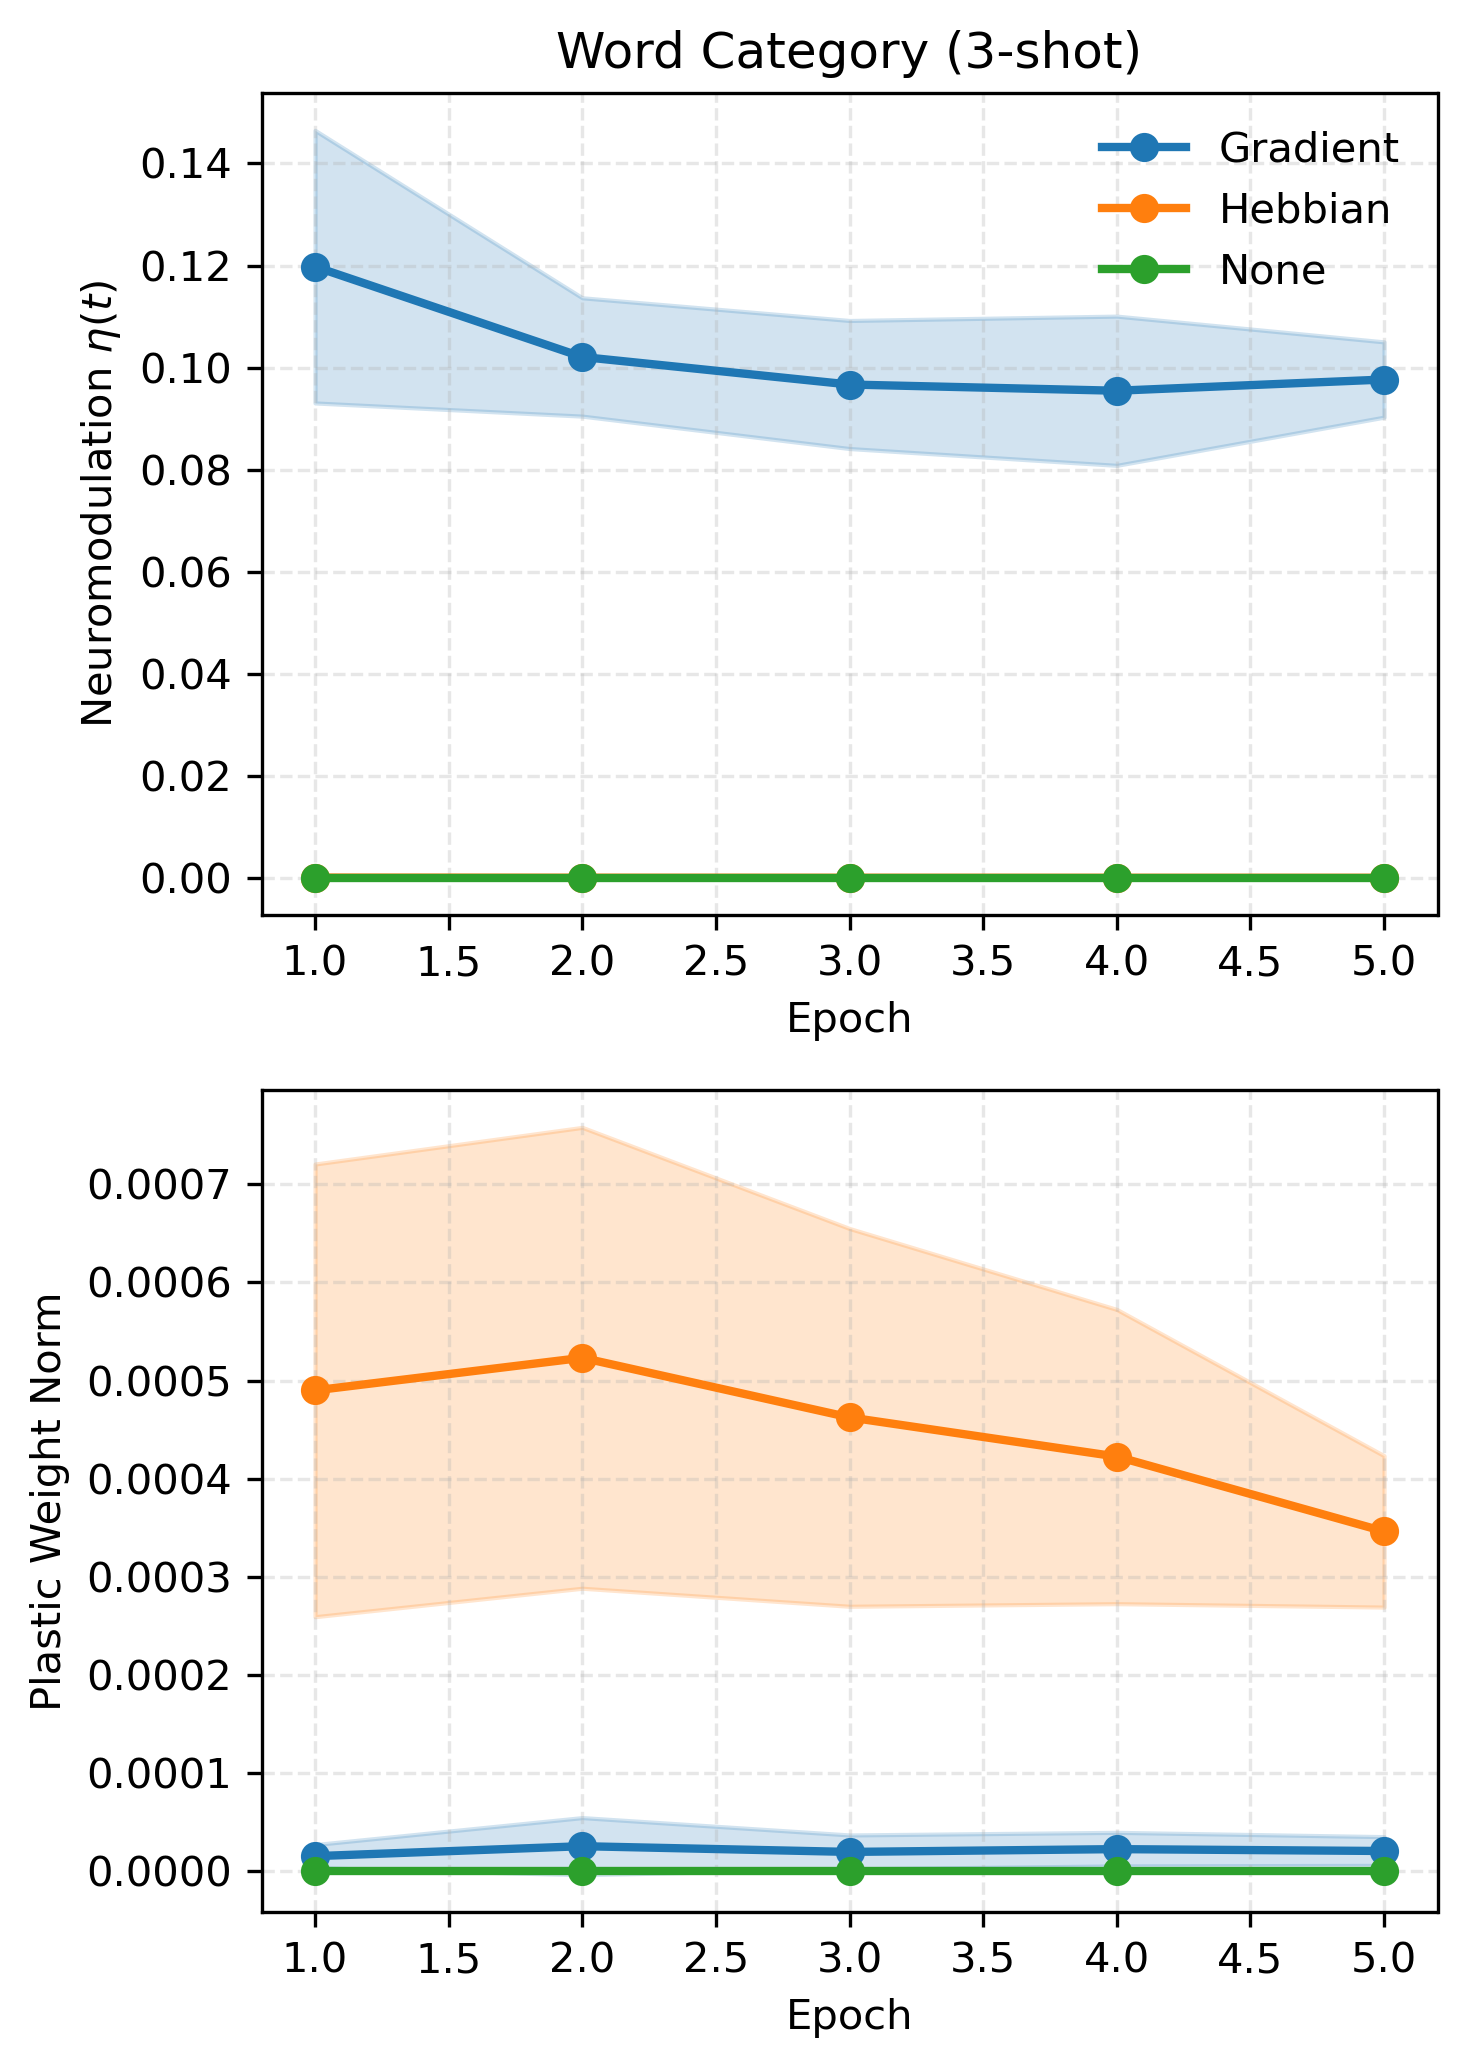
\includegraphics[width=\textwidth]{word_category_figures/word_category_mechanistic_traces.png}
        \caption{$\eta(t)$ and plastic weight norm}
        \label{fig:plot3}
    \end{subfigure}
    
    \caption{Results for Text Category Classification Experiment}
    \label{fig:Experiment 4 Results}
\end{figure}

\begin{table}[h]
    \centering
    \begin{tabular}{cccc} % No vertical lines (|) used here
        \toprule
        \textbf{RULE} & \textbf{ACCURACY} \\
        \midrule
        None & 0.609 $\pm$ 0.26  \\
        Hebbian & 0.429 $\pm$ 0.13 \\
       \textbf{Gradient} & \textbf{0.708} $\pm$ \textbf{0.27} \\
        \bottomrule
    \end{tabular}
    \caption{Three-Shot Text Category Classification Accuracy Results}
    \label{tab:Experiment 4 Table}
\end{table}

The Gradient rule performed the best, followed by the standard rule and the Hebbian rule. The Gradient rule was even able to achieve 100\% accuracy on one of the seeds. The wide error bars indicate that there was significant variance in accuracy across the seeds. Perhaps increased training metrics such as more epochs would reduce uncertainty in the accuracy. Additionally, the neuromodulation $\eta(t)$ was large for the Gradient rule, suggesting that this rule was able to classify the word categories well and update the fast weights quickly during the evaluation phase. 

%Test capacity by fixing size of weight matrix then increases training size, makes it recall the training data and records accuracy?

%Also a complicated idea that we can try to do that chatgpt came up is to try and merge gradient and hebbian descent into one model and let the model decide when to use what. I think this can be realized by adding another learnable feature that scales between the two delta w and try to learn that feature

\section{Comparison with Pre-trained Transformers}

We also tested how the Plastic transformers performed compared to large standard pre-trained transformers. For the Copying task and and Three-Shot Text Category task, we used the BERT base uncased model trained on English Wikipedia and BookCorpus, where the weights were kept fixed. For The One-Shot Image Classification task, we used the CLIP (Contrastive Language-Image Pre-training) model from OpenAI trained on image-text pairs.

Table \ref{tab:pre_trained results2} displays the results for the experiments, where bold indicates that a pre-trained model performed better than the Plastic transformer for both learning rules. 

\begin{table}[h]
    \centering
    \begin{tabular}{|c|c|c|c|}
        \hline
          Copying & Image Classification & Text Classification\\
        \hline
        0.0946 & \textbf{0.7843/0.6475}   & 0.6917 \\
        \hline
    \end{tabular}
    \caption{Test metrics for pre-trained transformers}
    \label{tab:pre_trained results2}
\end{table}

The BERT model performed poorly on the Copying Task relative to the previous models because this model does not have any weight updates. Thus, it cannot learn in-context. This means that pre-trained transformers need even further training to learn this task.

The CLIP model performed much better than the Plastic Transformer for the Image Classification task. This is likely due to the fact that it takes significant computational power and training data to train an image classification model, which the Plastic Transformer in this project did not have. 

The BERT model performed well on the Text Classification task, though slightly lower than the gradient plasticity model from previously. Below is a confusion matrix during the testing phase for the predicted classes, where the rows are the true category and the columns are the predicted category. The BERT model performed the highest on the animal category and the lowest on the furniture category.

\begin{table}[h!]
    \centering
    \begin{tabular}{|c|c|c|c|}
        \hline
           & Animals & Clothing & Furniture\\
        \hline
       Animals & 184 & 14 & 2\\
       \hline
       Clothing & 42 & 153 & 5\\
       \hline
       Furniture & 58 & 64 & 78 \\
        \hline
    \end{tabular}
    \caption{Confusion Matrix for Experiment 3 (Three-Shot Text Category Classification task)}
    \label{tab:pre_trained results}
\end{table}



\section{Analysis of Results}

The performance tasks in the original paper only used a very small model and ran through very limited epochs. Moreover, the test results stopped at only around 0.3 accuracy for the One-Shot Image Classification task. Our hypothesis is that Hebbian Plasticity seems to dominate because the outer product weight update quickly adapted to the example using local information, while the Gradient Rule works more slowly towards the end goal.

If we increase the training epochs, or make the problem more complex e.g. The Three-Shot Text Category Classification task, we find that the Gradient Method becomes the dominating method.

Other than accuracy boosts, we conducted a capacity test on the Copying task by training the model on varying signal length. We find that in this scenario, the plasticity weights seem to stabilize behavior across random seeds.

By comparing to large Pre-Trained Transformers BERT and CLIP, trained on large amount of text and image data, respectively, we find that these Pre-Trained Transformer performed much better in text classification and image classification, respectively, while they did very poorly on the Copying Task. This is expected, since the Pre-trained Transformers do not have any weight updates during evaluation, they perform poorly on tasks they have not been trained on.

In the results we obtained, the Gradient Plasticity Method seems to perform the best of the three in general cases.

%In the One-Shot Image Classfication task, a task with a very small training set, Hebbian Plasticity dominated because the outer product weight update recorded the example directly into the weights, allowing the model to recognize an unlabeled example later. Additionally, the neuromodulation factor was relatively small for the Hebbian update, meaning that the Transformer did not require huge plasticity signals to work well under this update rule.

%However, in the Three-Shot Text Category Classification task this was not the case, even though more training samples were provided. This suggests that the Hebbian rule works better in situations where the data samples provide lots of information, like image data, while the gradient rule could work better in situations where data examples provide less information. 

\newpage
\bibliographystyle{plain}
\bibliography{cite.bib}

\end{document}
